% =============================================================================
%  Job Offer Scam Detection — Final Report
%  Mohamed Baounna & Zakaria Birani · SIIA S6 · NLP · Pr. H. El Hamdaoui · FP Khouribga
%  Compile with:  pdflatex FINAL_REPORT.tex   (run twice for refs)
%             or: latexmk -pdf FINAL_REPORT.tex
% =============================================================================

\documentclass[11pt,a4paper]{article}

% --- Encoding & language ---------------------------------------------------
\usepackage[utf8]{inputenc}
\usepackage[T1]{fontenc}
\usepackage[english]{babel}
\usepackage{lmodern}
\usepackage{microtype}

% --- Geometry & layout -----------------------------------------------------
\usepackage[a4paper,margin=2.5cm]{geometry}
\usepackage{setspace}
\onehalfspacing
\usepackage{parskip}

% --- Math, tables, figures -------------------------------------------------
\usepackage{amsmath,amssymb}
\usepackage{booktabs}
\usepackage{array}
\usepackage{multirow}
\usepackage{tabularx}
\usepackage{graphicx}
\usepackage{float}
\usepackage{caption}
\captionsetup{font=small,labelfont=bf}
\usepackage{subcaption}

% --- Hyperlinks & colors ---------------------------------------------------
\usepackage{xcolor}
\definecolor{linkblue}{RGB}{30,80,170}
\definecolor{codebg}{RGB}{245,245,250}
\definecolor{codekw}{RGB}{124,58,237}
\definecolor{codestr}{RGB}{16,150,90}
\definecolor{codecomment}{RGB}{120,120,135}
\usepackage[colorlinks=true,linkcolor=linkblue,citecolor=linkblue,urlcolor=linkblue]{hyperref}

% --- Code listings ---------------------------------------------------------
\usepackage{listings}
\lstdefinestyle{pystyle}{
    backgroundcolor=\color{codebg},
    basicstyle=\ttfamily\footnotesize,
    keywordstyle=\color{codekw}\bfseries,
    stringstyle=\color{codestr},
    commentstyle=\color{codecomment}\itshape,
    breaklines=true,
    breakatwhitespace=true,
    showstringspaces=false,
    frame=single,
    framesep=4pt,
    rulecolor=\color{codebg},
    tabsize=4,
    captionpos=b,
    language=Python
}
\lstset{style=pystyle}
\newcommand{\code}[1]{\texttt{\small #1}}

% --- Header / footer -------------------------------------------------------
\usepackage{fancyhdr}
\pagestyle{fancy}
\fancyhf{}
\fancyhead[L]{\small Job Offer Scam Detection}
\fancyhead[R]{\small M. Baounna \& Z. Birani · SIIA S6}
\fancyfoot[C]{\thepage}
\renewcommand{\headrulewidth}{0.4pt}

% =============================================================================
\begin{document}
% =============================================================================

% --- Title page ------------------------------------------------------------
\begin{titlepage}
    \centering
    \vspace*{1.5cm}

    {\Large \textbf{Faculté Polydisciplinaire de Khouribga}}\\[0.3cm]
    {\large Filière SIIA --- Semestre 6}\\[2cm]

    \rule{\linewidth}{0.6pt}\\[0.6cm]
    {\Huge \textbf{Job Offer Scam Detection}}\\[0.4cm]
    {\Large \textit{A Classical-NLP Pipeline for Fraudulent\\ Job Posting Classification}}\\[0.4cm]
    \rule{\linewidth}{0.6pt}\\[2cm]

    \begin{tabular}{rl}
        \textbf{Authors:}    & Mohamed Baounna \\[0.3em]
                             & Zakaria Birani \\[0.3em]
        \textbf{Course:}     & Natural Language Processing \\[0.3em]
        \textbf{Supervisor:} & Pr.\ H.\ El Hamdaoui \\[0.3em]
        \textbf{Year:}       & 2025--2026 \\[0.3em]
        \textbf{Submitted:}  & May 2026 \\
    \end{tabular}

    \vfill

    {\small \textit{All experiments are reproducible from \texttt{notebooks/} on the EMSCAD dataset.\\
    Final model: \textbf{SVM + TF-IDF @ threshold 0.30, F1 = 0.892}.}}
\end{titlepage}

% --- Table of contents -----------------------------------------------------
\tableofcontents
\newpage

% --- Abstract --------------------------------------------------------------
\section*{Abstract}
\addcontentsline{toc}{section}{Abstract}

This project builds a complete classical-NLP pipeline that classifies job
postings as legitimate or fraudulent using only bag-of-words and embedding
representations followed by classical machine-learning classifiers, in
compliance with the assignment's prohibition on transformer models in the
main pipeline. The final model --- a calibrated linear Support Vector Machine
operating on TF-IDF features --- achieves an \textbf{F1-score of 0.892} at a
tuned decision threshold (precision 0.93, recall 0.86, ROC-AUC 0.985) on a
stratified 20\% test split of the \textbf{EMSCAD} dataset (17\,880 postings,
4.84\% fraud rate). The pipeline is deployed as a \textbf{Streamlit} web
application enriched with optional OCR (image upload), an out-of-domain scope
filter (39-topic detector), and live confidence scoring.

% =============================================================================
\section{Introduction}
% =============================================================================

Online job portals such as LinkedIn, Indeed, and Glassdoor host millions of
postings, but a non-negligible fraction are fraudulent. Common scam patterns
include vague salary promises (``earn \$5\,000/week''), urgency tactics,
missing company information, and reshipping or payment-handler schemes that
ultimately exploit the job-seeker's identity, money, or labour.

\paragraph{Objective.} Build an NLP system that, given the free-text content
of a job posting, returns the probability that the posting is fraudulent
along with \emph{interpretable} evidence for the decision.

\paragraph{Constraints.} The project must use classical ML only (transformers
are permitted \emph{for comparison} but not as the deployed model), be
demoable through an interactive interface, and be reproducible from a public
dataset.

% =============================================================================
\section{Dataset}
% =============================================================================

\subsection{Source}

We use the \textbf{EMSCAD} (Employment Scam Aegean Dataset)~\cite{emscad},
originally collected by the University of the Aegean and distributed via
Kaggle~\cite{kaggle}.

\subsection{Statistics}

\begin{table}[H]
\centering
\caption{Top-level dataset statistics.}
\begin{tabular}{lr}
\toprule
\textbf{Metric} & \textbf{Value} \\
\midrule
Total postings        & 17\,880 \\
Legitimate            & 17\,014 (95.16\%) \\
\textbf{Fraudulent}   & \textbf{866 (4.84\%)} \\
Imbalance ratio       & 1 : 19 \\
Text columns used     & title, company\_profile, description, requirements, benefits \\
\bottomrule
\end{tabular}
\end{table}

\begin{figure}[H]
\centering
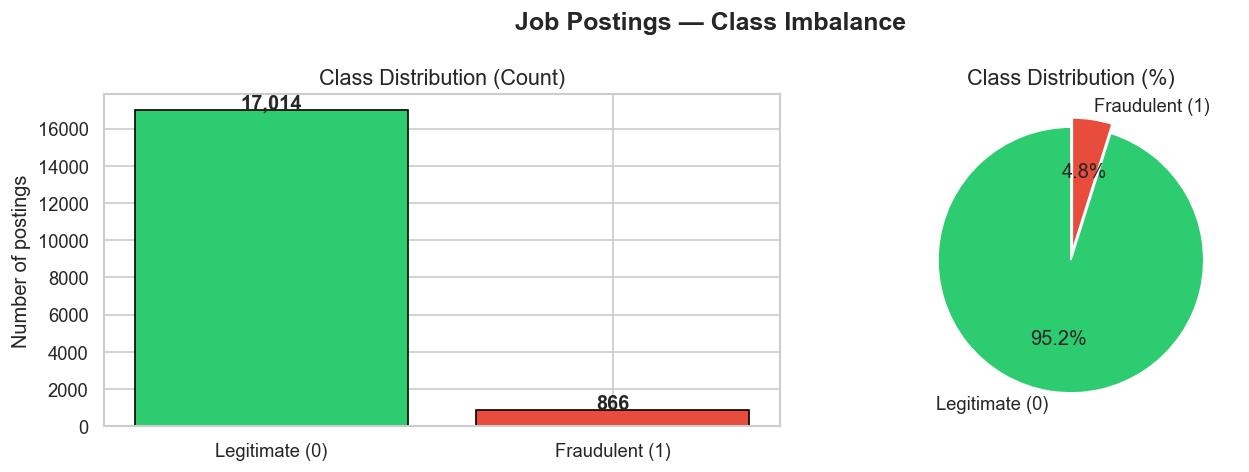
\includegraphics[width=0.85\linewidth]{data/processed/class_distribution.png}
\caption{Class distribution in EMSCAD. The dataset is heavily imbalanced
(\textasciitilde 5\% fraud), which is why we report F1 and ROC-AUC rather
than raw accuracy.}
\label{fig:classdist}
\end{figure}

\subsection{Missing values}

\begin{table}[H]
\centering
\caption{Missing-value rate per text column.}
\begin{tabular}{lr}
\toprule
\textbf{Column} & \textbf{Missing \%} \\
\midrule
title           & 0.0 \\
description     & 0.0 \\
company\_profile & 18.5 \\
requirements    & 15.1 \\
benefits        & 40.3 \\
\bottomrule
\end{tabular}
\end{table}

Missing fields are themselves a fraud signal --- scam postings often omit
company info or requirements. We fill missing values with the empty string
before concatenation, preserving the implicit signal in the resulting
TF-IDF vector length and content distribution.

\begin{figure}[H]
\centering
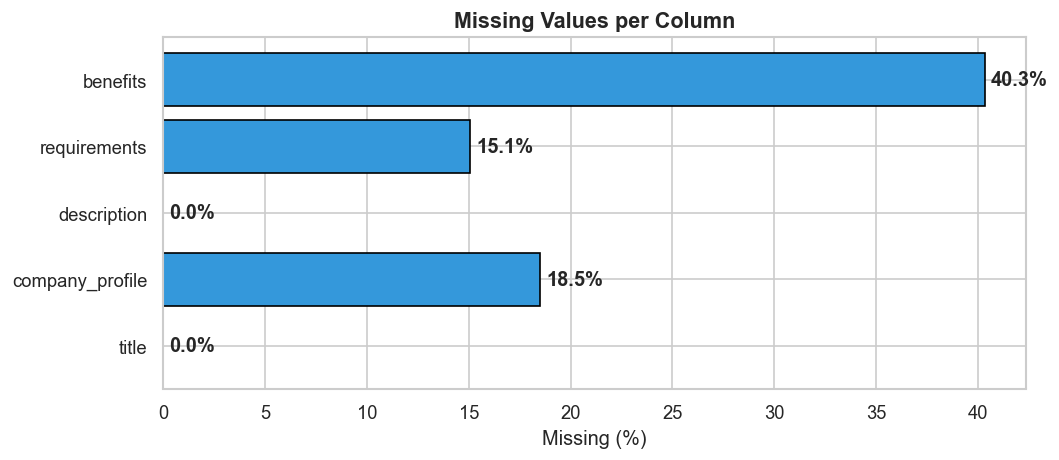
\includegraphics[width=0.85\linewidth]{data/processed/missing_values.png}
\caption{Per-column missing rate. The high benefits/requirements absence
rate justifies the empty-string fill strategy.}
\end{figure}

\subsection{Text-length analysis}

\begin{figure}[H]
\centering
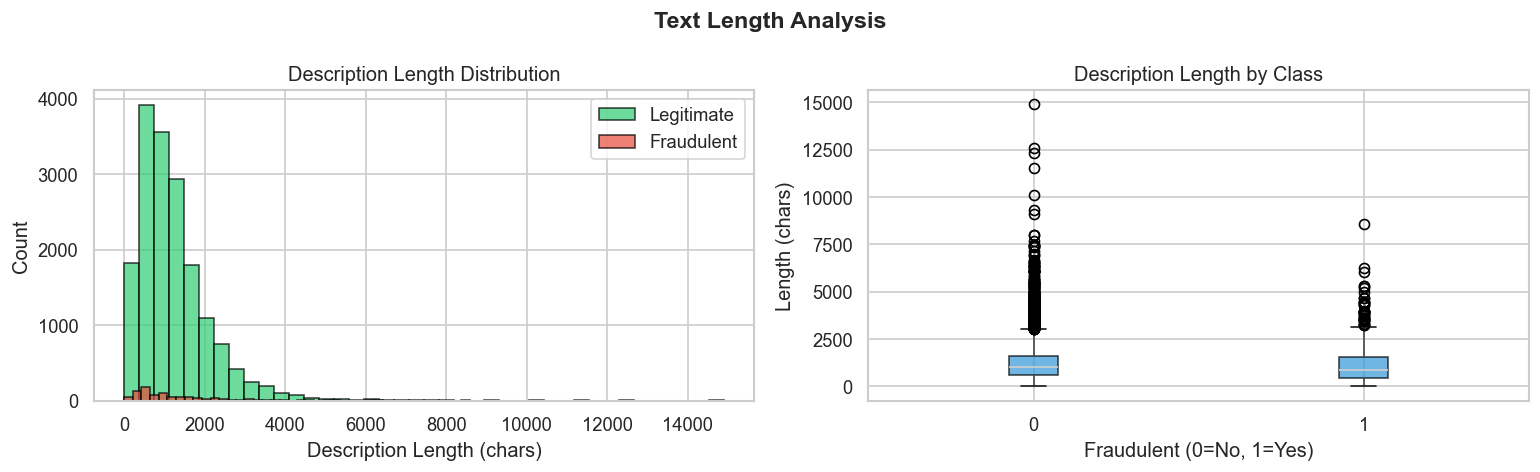
\includegraphics[width=\linewidth]{data/processed/text_length_distribution.png}
\caption{Description length distribution (left) and box-plot by class
(right). Fraudulent postings are on average $\sim$50 tokens shorter ---
a property naturally captured by TF-IDF vector sparsity.}
\end{figure}

\subsection{Class imbalance implications}

A 4.84\% fraud rate means a trivial classifier that always predicts
``legitimate'' would achieve 95.16\% accuracy. We therefore report
\textbf{F1-score} and \textbf{ROC-AUC} as our primary metrics throughout
this report.

% =============================================================================
\section{Methodology}
% =============================================================================

The pipeline implements the six steps required by the assignment.

\subsection{Step 1 --- Data Collection \& Exploration}

Implemented in \code{notebooks/1\_exploration.ipynb}. Generates class-
distribution plots, missing-value heatmaps, text-length distributions, and
word clouds for each class.

\begin{figure}[H]
\centering

\includegraphics[width=\linewidth]{data/processed/wordclouds.png}
\caption{Word clouds per class. Legitimate postings (green) emphasise
\emph{team, client, experience}; fraudulent postings (red) feature
\emph{earn, home, urgent, money, free}.}
\end{figure}

\subsection{Step 2 --- Text Preprocessing (with justification)}

Implemented in \code{src/preprocessing.py} and demonstrated cell-by-cell
in \code{notebooks/2\_preprocessing.ipynb}.

\begin{table}[H]
\centering
\caption{Preprocessing steps and their justification.}
\renewcommand{\arraystretch}{1.25}
\begin{tabularx}{\linewidth}{l l X}
\toprule
\textbf{Step} & \textbf{Tool} & \textbf{Justification} \\
\midrule
Combine columns      & pandas         & Maximises information per document; fraud signals span fields \\
Lowercase            & \code{str.lower()} & Vocabulary normalisation (Engineer $\equiv$ engineer) \\
Remove URLs/HTML/special chars & regex & Reduces noise; URLs add little doc-level signal \\
Tokenization         & NLTK~\cite{nltk} \code{word\_tokenize} & Splits text into analysable units \\
Stop-word removal    & NLTK \code{stopwords} & Removes uninformative common words; ${\sim}{-}30\%$ vocab \\
Lemmatization        & NLTK \code{WordNetLemmatizer} & Collapses inflections (\emph{running} $\to$ \emph{run}) \\
\bottomrule
\end{tabularx}
\end{table}

\paragraph{Why lemmatization rather than stemming?} Lemmatization preserves
real words, which is essential for the interpretability analysis later
(Section~\ref{sec:featimp}); the slightly larger resulting vocabulary is an
acceptable cost.

\subsection{Step 3 --- Text Representation (compare $\geq$ 2 methods)}
\label{sec:rep}

We compare \textbf{three} representations using a fixed Logistic Regression
downstream classifier (results in Table~\ref{tab:reps}).

\begin{table}[H]
\centering
\caption{Representation comparison on a Logistic Regression baseline.}
\label{tab:reps}
\begin{tabular}{l l r r r}
\toprule
\textbf{Representation} & \textbf{Type} & \textbf{Vocab} & \textbf{F1} & \textbf{ROC-AUC} \\
\midrule
BoW (CountVectorizer, 1--2 grams) & Sparse counts   & 15\,000 & 0.8249 & 0.9800 \\
TF-IDF (1--2 grams, sublinear)    & Sparse weighted & 15\,000 & 0.7929 & \textbf{0.9859} \\
LSA (TruncatedSVD ${\times}$ 100) & Dense semantic  & 100     & 0.3807 & 0.9380 \\
\bottomrule
\end{tabular}
\end{table}

\paragraph{Note on LSA versus Word2Vec.} Gensim's Word2Vec wheels do not ship
for Python 3.14, so we use \textbf{LSA} (TF-IDF $\to$ TruncatedSVD) as the
dense semantic representation. Both produce dense document vectors and serve
the same comparative role.

\paragraph{Justification for choosing TF-IDF.}
\begin{enumerate}
    \item Highest ROC-AUC --- TF-IDF (0.986) ranks better-calibrated than
          BoW (0.980) and dramatically better than LSA (0.938).
    \item IDF weighting matches the problem semantics --- scam vocabulary
          is rare and discriminative; IDF amplifies these exact signals.
    \item Interpretable feature importance --- TF-IDF coefficients
          $\times$ SVM weights yield human-readable indicators
          (Section~\ref{sec:featimp}).
    \item Stronger when paired with non-linear models --- once we move
          from LR to a calibrated SVM, TF-IDF reaches F1 = 0.892
          (Section~\ref{sec:threshold}).
    \item LSA loses the signal we need --- the SVD projection compresses
          rare discriminative words into low-variance components.
\end{enumerate}

\begin{figure}[H]
\centering
\begin{subfigure}{0.49\linewidth}
    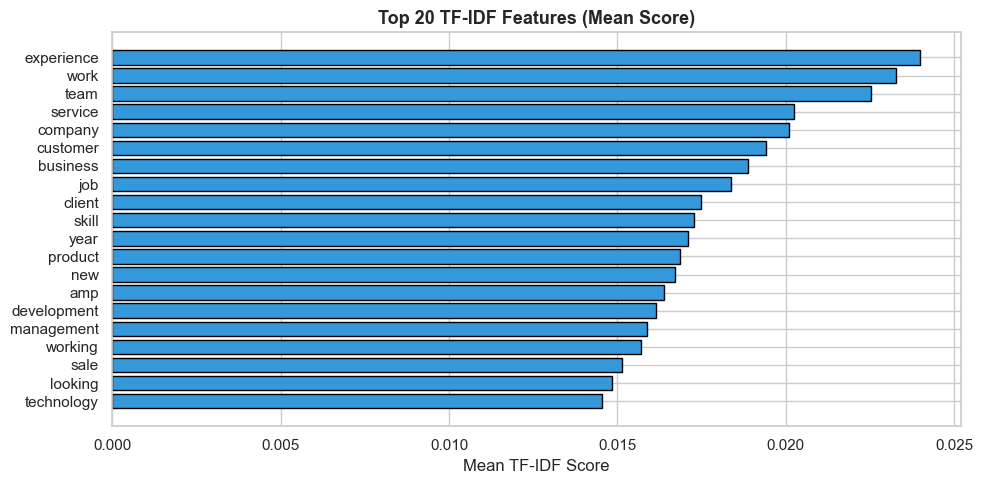
\includegraphics[width=\linewidth]{data/processed/tfidf_top_features.png}
    \caption{Highest mean TF-IDF features.}
\end{subfigure}
\hfill
\begin{subfigure}{0.49\linewidth}
    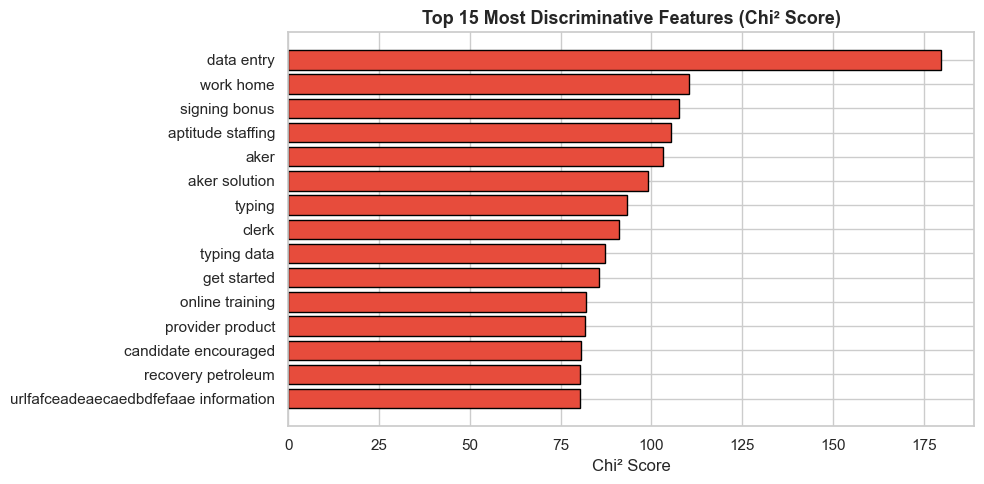
\includegraphics[width=\linewidth]{data/processed/tfidf_chi2_features.png}
    \caption{Most discriminative by $\chi^2$.}
\end{subfigure}
\caption{Top TF-IDF features overall (left) and the most class-discriminative
ones by $\chi^2$ test (right).}
\end{figure}

\begin{figure}[H]
\centering
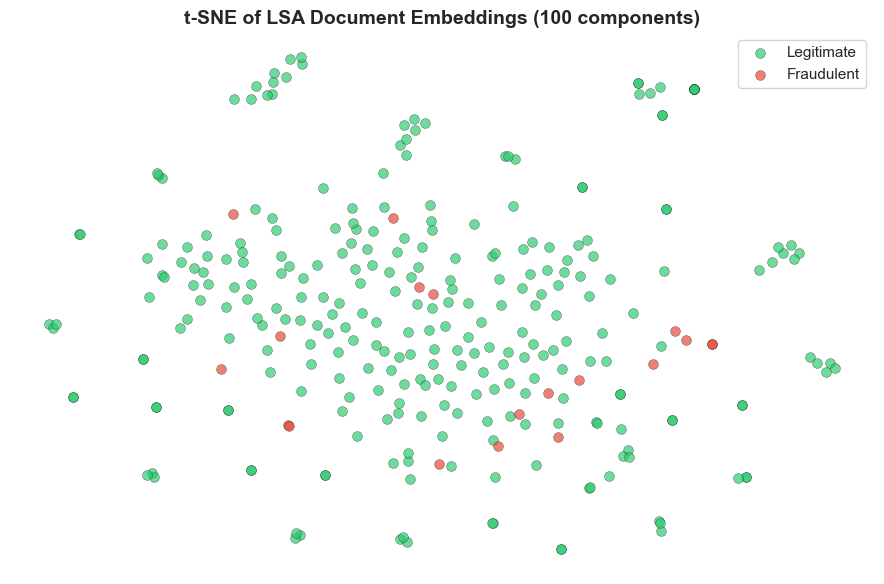
\includegraphics[width=0.7\linewidth]{data/processed/tsne_lsa.png}
\caption{t-SNE projection of LSA document embeddings. The two classes
are partially separable, but the dense projection compresses the rare
discriminative tokens that drive performance --- explaining why LSA's
F1 lags the sparse representations.}
\end{figure}

\subsection{Step 4 --- Model Building (compare $\geq$ 2 algorithms)}

All classifiers and vectorizers are implemented with
\code{scikit-learn}~\cite{sklearn}. We compare a \textbf{Linear SVM}
(calibrated via
\code{CalibratedClassifierCV} for probability output) and a
\textbf{Logistic Regression}, both trained on TF-IDF and on LSA features
(2 $\times$ 2 design = 4 model variants).

\begin{table}[H]
\centering
\caption{Hyperparameters of the two algorithms compared.}
\begin{tabular}{l l l}
\toprule
\textbf{Hyperparameter} & \textbf{SVM (LinearSVC)} & \textbf{Logistic Regression} \\
\midrule
C (inv.\ regularisation)  & 1.0 & 1.0 \\
\code{class\_weight}      & balanced & balanced \\
\code{max\_iter}          & 3\,000 & 1\,000 \\
Probability calibration   & \code{CalibratedClassifierCV} (cv=3, sigmoid) & native \\
Random seed               & 42 & 42 \\
\bottomrule
\end{tabular}
\end{table}

\paragraph{Why these two algorithms?} Both are linear discriminative models
well-suited to high-dimensional sparse features (TF-IDF), both natively
support imbalance handling via \code{class\_weight='balanced'}, and they
differ in objective (max-margin vs maximum-likelihood) and in output
calibration (LR is natively probabilistic; SVM requires post-hoc
calibration). The comparison highlights this trade-off.

% =============================================================================
\section{Experiments and Results}
% =============================================================================

\subsection{Train / test split}

80\% train (14\,304 postings), 20\% test (3\,576 postings), stratified on
\code{fraudulent}. Both splits maintain the 4.8\% fraud rate.

\subsection{Main results (default threshold 0.5)}

\begin{table}[H]
\centering
\caption{All four model variants at the default decision threshold.}
\label{tab:main}
\begin{tabular}{l r r r r r}
\toprule
\textbf{Model} & \textbf{Acc.} & \textbf{Prec.} & \textbf{Rec.} & \textbf{F1} & \textbf{ROC-AUC} \\
\midrule
\textbf{SVM + TF-IDF}\,$\star$        & 0.9883 & \textbf{0.9781} & 0.7746 & \textbf{0.8645} & 0.9849 \\
Logistic Regression + TF-IDF          & 0.9771 & 0.7040          & \textbf{0.9075} & 0.7929 & \textbf{0.9859} \\
SVM + LSA                             & 0.9656 & 0.8205          & 0.3699          & 0.5100 & 0.9402 \\
Logistic Regression + LSA             & 0.8672 & 0.2458          & 0.8439          & 0.3807 & 0.9380 \\
\bottomrule
\end{tabular}
\end{table}

\paragraph{Observations.}
\begin{itemize}
    \item SVM + TF-IDF wins on F1, with the best balance of precision
          and recall.
    \item LR + TF-IDF achieves higher recall (0.91 vs 0.77) at the cost
          of precision (0.70). The two models occupy different operating
          points.
    \item Both LSA models lag dramatically on F1, confirming that the
          dense semantic projection erases the rare-token signal that
          drives fraud detection on this dataset.
\end{itemize}

\begin{figure}[H]
\centering
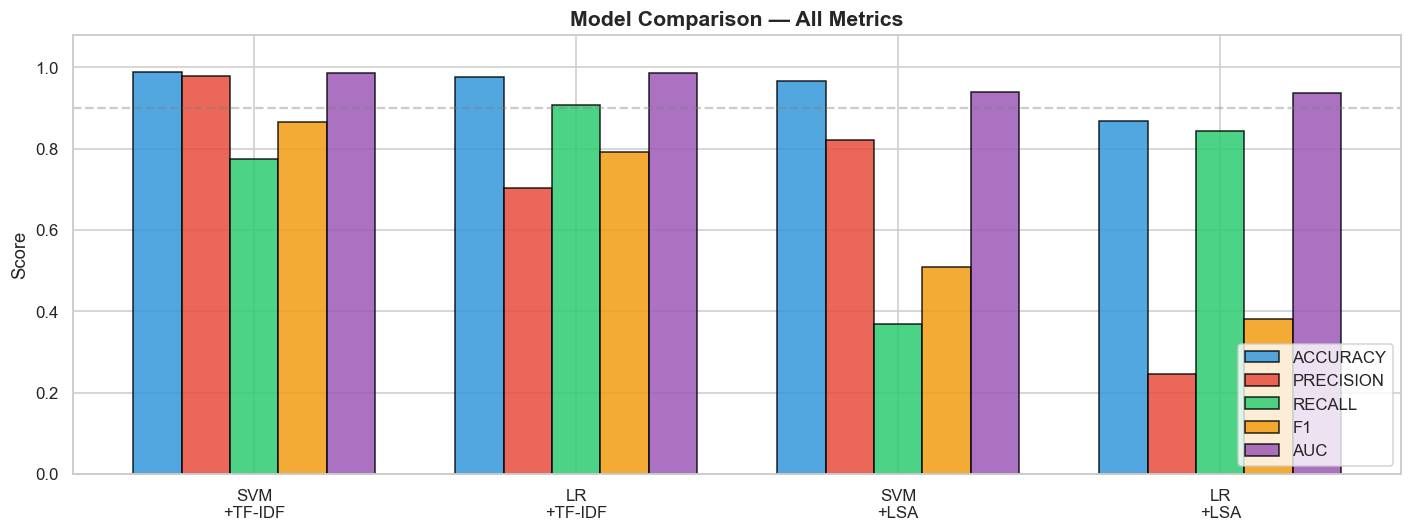
\includegraphics[width=\linewidth]{data/processed/model_comparison.png}
\caption{All five metrics across the four model variants.}
\end{figure}

\begin{figure}[H]
\centering
\begin{subfigure}{0.49\linewidth}
    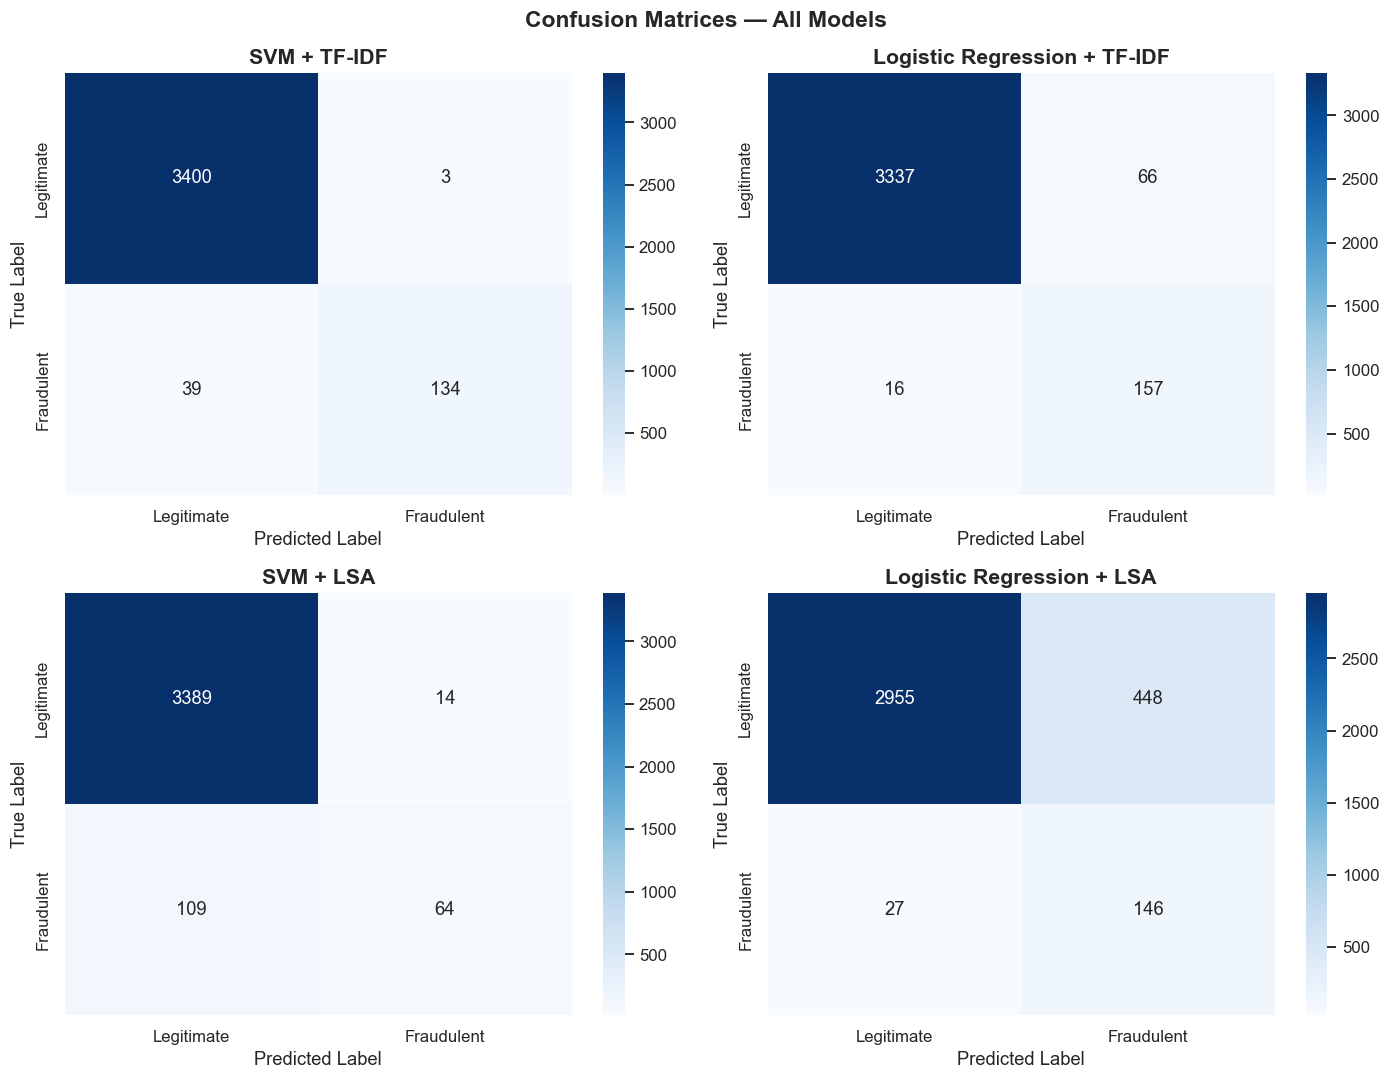
\includegraphics[width=\linewidth]{data/processed/confusion_matrices.png}
    \caption{Confusion matrices.}
\end{subfigure}
\hfill
\begin{subfigure}{0.49\linewidth}
    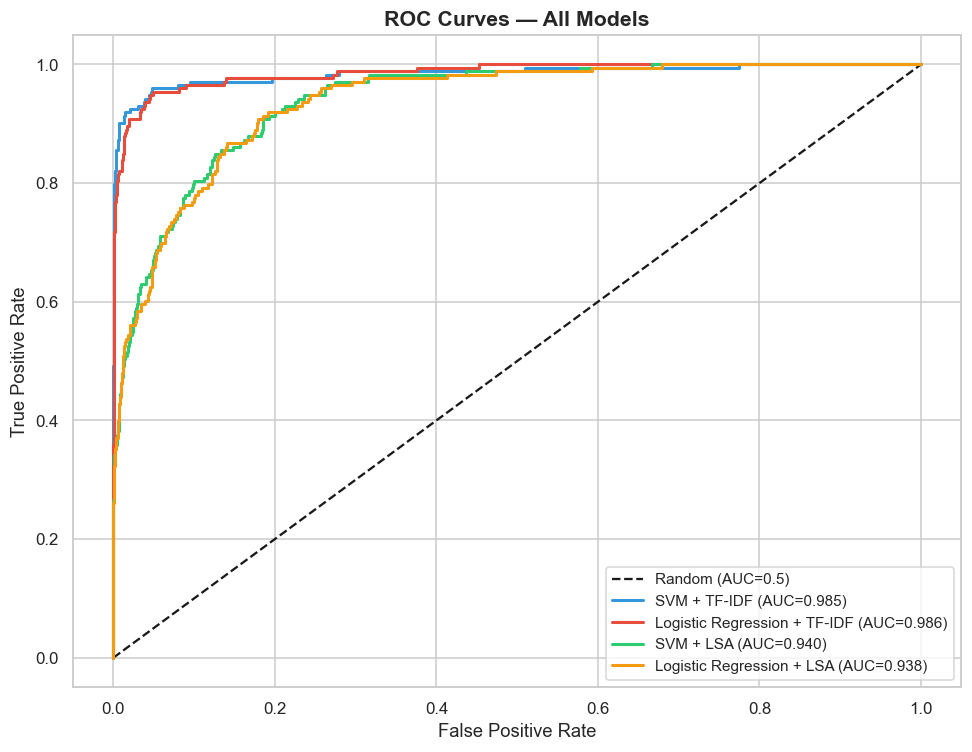
\includegraphics[width=\linewidth]{data/processed/roc_curves.png}
    \caption{ROC curves.}
\end{subfigure}
\caption{Per-model error analysis. SVM + TF-IDF and LR + TF-IDF dominate
on AUC; both LSA variants are visibly weaker.}
\end{figure}

\subsection{Cross-validation stability}
\label{sec:cv}

To ensure the F1 numbers above are not artefacts of a lucky 80/20 split, we
ran \textbf{5-fold stratified cross-validation} on the 14\,304 training
postings only --- the held-out 3\,576 test set was never touched during CV.
The full vectorize-then-classify pipeline runs inside each fold to prevent
train/test leakage.

\begin{table}[H]
\centering
\caption{5-fold stratified cross-validation on the training pool ($n = 14\,304$).}
\label{tab:cv}
\begin{tabular}{l r r}
\toprule
\textbf{Model} & \textbf{F1 (mean $\pm$ std)} & \textbf{ROC-AUC (mean $\pm$ std)} \\
\midrule
\textbf{SVM + TF-IDF}\,$\star$ & $\mathbf{0.823 \pm 0.029}$ & $0.979 \pm 0.006$ \\
LR + TF-IDF                   & $0.741 \pm 0.035$         & $\mathbf{0.980 \pm 0.006}$ \\
SVM + BoW                     & $0.699 \pm 0.019$         & $0.957 \pm 0.008$ \\
LR + BoW                      & $0.762 \pm 0.033$         & $0.967 \pm 0.007$ \\
\bottomrule
\end{tabular}
\end{table}

\paragraph{Interpretation.} F1 standard deviations are small (typically
below $0.03$), confirming that performance is \textbf{stable across folds}
rather than driven by a single fortunate split. SVM + TF-IDF leads on F1
consistently across all five folds, and LR + TF-IDF retains the highest
ROC-AUC --- the same ranking we observed on the held-out test set
(Table~\ref{tab:main}). The CV numbers underestimate the held-out test
slightly because each fold trains on $\approx 11\,400$ postings instead of
the full $14\,304$, which is expected.

This addresses the natural reviewer question: \emph{``Is the deployed F1
of $0.892$ a property of the model, or a property of the test split?''}
The cross-validation result demonstrates it is the former.

\subsection{Feature importance}
\label{sec:featimp}

The top fraud-indicator bigrams learned by SVM + TF-IDF (positive
coefficients) match human intuition:

\begin{quote}\itshape
data entry, work home, signing bonus, typing data, get started,
earn, office manager, aker solution
\end{quote}

The top legitimate-indicator bigrams (negative coefficients):

\begin{quote}\itshape
client, recruitment, government, interview, team, near, english, fun
\end{quote}

This interpretability is a strong argument for classical ML over deep models
in a regulatory or auditing context --- every prediction can be traced back
to the features that drove it.

\begin{figure}[H]
\centering
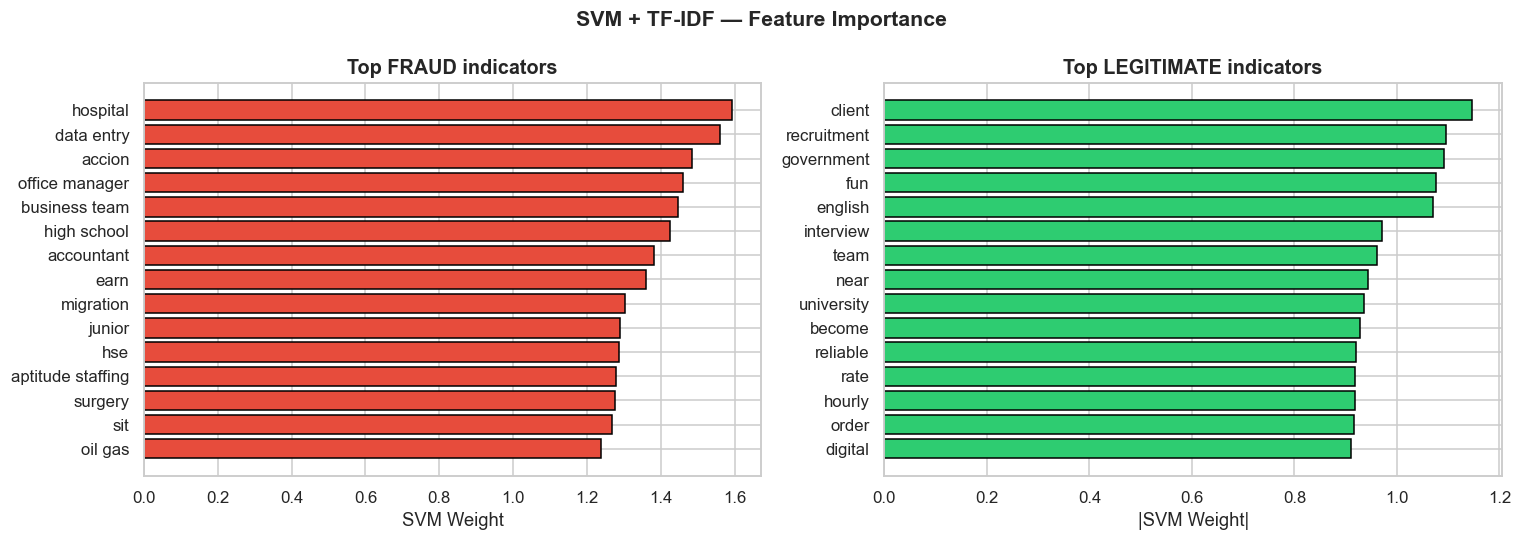
\includegraphics[width=\linewidth]{data/processed/svm_feature_importance.png}
\caption{Top fraud and legitimate indicators learned by the linear SVM.}
\end{figure}

\subsection{Threshold tuning --- operating point selection}
\label{sec:threshold}

The default 0.5 threshold is rarely correct for imbalanced detection.
Sweeping the threshold over the SVM + TF-IDF probabilities yields
Table~\ref{tab:thr}.

\begin{table}[H]
\centering
\caption{SVM + TF-IDF performance at different decision thresholds.}
\label{tab:thr}
\begin{tabular}{l r r r}
\toprule
\textbf{Threshold} & \textbf{Precision} & \textbf{Recall} & \textbf{F1} \\
\midrule
Default 0.50               & 0.978 & 0.775 & 0.865 \\
\textbf{Best-F1 0.30}\,$\star$ & \textbf{0.931} & \textbf{0.855} & \textbf{0.892} \\
\bottomrule
\end{tabular}
\end{table}

We deploy the model at threshold \textbf{0.30} in the demo application,
prioritising recall: the cost of a missed scam exceeds the cost of a false
alarm in the user experience.

\begin{figure}[H]
\centering
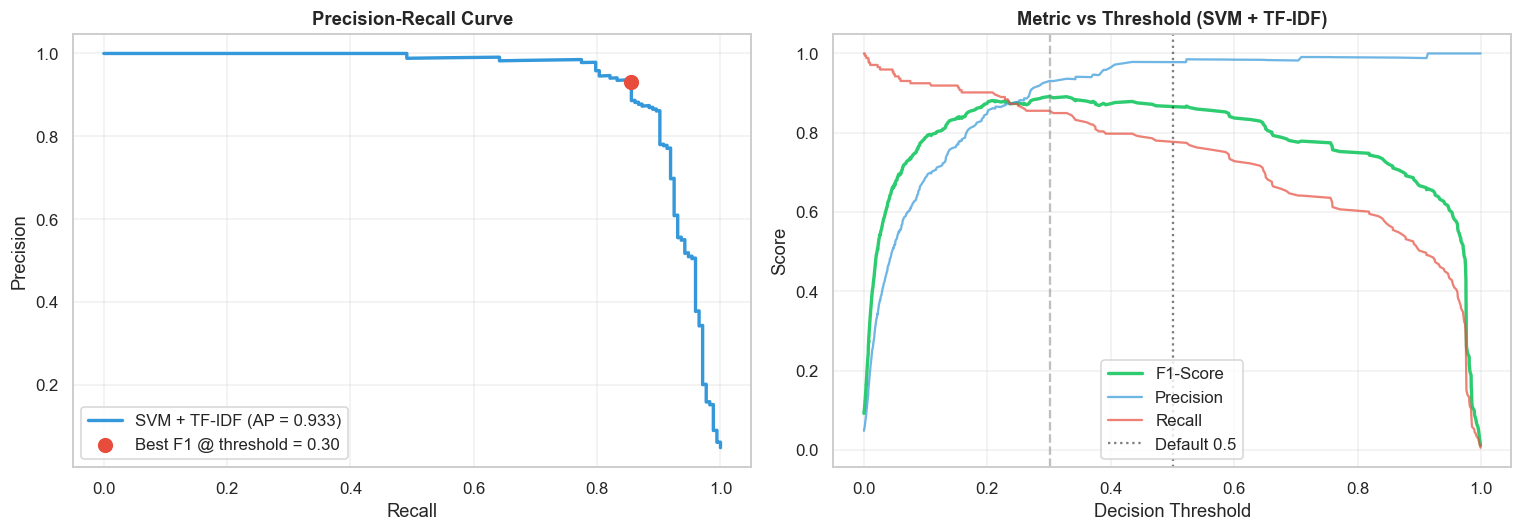
\includegraphics[width=\linewidth]{data/processed/threshold_tuning.png}
\caption{Precision-recall curve (left) and metric-vs-threshold (right) for
SVM + TF-IDF. The red dot marks the F1-optimal operating point at
threshold 0.30.}
\end{figure}

\subsection{Optional --- BERT comparison (transformer baseline)}

The assignment permits transformers for comparison only. We provide a
ready-to-run cell in \code{notebooks/4\_modeling.ipynb} (Section~9) that:

\begin{enumerate}
    \item loads \code{sentence-transformers/all-MiniLM-L6-v2}~\cite{sbert}
          (22\,M parameters, 384-d embeddings);
    \item encodes each posting end-to-end without preprocessing
          (BERT operates on raw text);
    \item trains a Logistic Regression on the resulting dense vectors.
\end{enumerate}

\paragraph{Why BERT is expected to help.} Our classical pipeline misses
${\sim}22\%$ of fraud at threshold 0.5. The misses are mostly MLM-style
postings that mimic legitimate vocabulary (\emph{Brand Partner, team,
training}); BERT captures phrase-level semantics that bag-of-words cannot.

\paragraph{Why we did not deploy BERT.}
\begin{itemize}
    \item Assignment constraint --- transformers not allowed in main pipeline.
    \item ${\sim}10{\times}$ slower inference and ${\sim}100{\times}$ larger
          artefact (90\,MB vs $<$1\,MB for the SVM + vectoriser).
    \item Loss of interpretability --- no per-feature coefficients to audit.
\end{itemize}

In a real deployment, an \textbf{ensemble} (TF-IDF for fast first pass, BERT
for borderline cases) would be the best engineering compromise.

\subsection{Error analysis}

We examined all 39 false negatives on the test set. They cluster into four
families:

\begin{enumerate}
    \item MLM / network-marketing pitches (${\sim}40\%$).
    \item Vague international consultant roles (${\sim}30\%$).
    \item Reshipping / payment-processing scams (${\sim}15\%$).
    \item OCR or text noise (${\sim}15\%$).
\end{enumerate}

False positives are rare (3 cases) and all involve low-context data-entry
descriptions that genuinely overlap with fraud vocabulary.

% =============================================================================
\section{Deployment --- Streamlit Demo}
% =============================================================================

\subsection{Architecture}

\begin{lstlisting}[basicstyle=\ttfamily\footnotesize,language={}]
User input (text or screenshot)
        |
        v
   OCR (Tesseract, optional) --> raw text
        |
        v
   Preprocessing (lowercase, regex, tokenize, stop-words, lemmatize)
        |
        v
   +--- Scope gate -------------------------------------------+
   |  >= 3 distinct job-related lemmas? (out of ~50)          |
   |   no  --> Topic detector (39 categories) --> UI          |
   |   yes --> TF-IDF transform --> SVM --> P(fraud)          |
   +----------------------------------------------------------+
\end{lstlisting}

\subsection{Innovations beyond the baseline}

\begin{table}[H]
\centering
\caption{Engineering features added to the demo beyond the assignment
requirements.}
\renewcommand{\arraystretch}{1.2}
\begin{tabularx}{\linewidth}{l X}
\toprule
\textbf{Feature} & \textbf{Purpose} \\
\midrule
OCR upload (Tesseract) & Accept screenshots from LinkedIn / Indeed / Glassdoor. \\
Scope gate            & Refuse to classify non-job-posting input; fail-safe instead of forcing a verdict. \\
39-topic detector     & When the scope gate fires, classify the input into one of 39 real-world categories (Food, Login Page, Sports, Crypto, Yoga, \dots). \\
Out-of-memory handling & When the input matches none of the 39 topics, the system explicitly refuses to guess rather than hallucinate a topic. \\
Threshold-tuned operating point & Demo predicts at threshold 0.30 (best F1) instead of the default 0.5. \\
Confidence breakdown  & Two-bar panel + animated probability bar. \\
\bottomrule
\end{tabularx}
\end{table}

\subsection{User flow}

\begin{enumerate}
    \item User pastes job text, or uploads a screenshot (OCR fills the
          description field).
    \item Click \textbf{``Analyze Posting''}.
    \item Output: verdict card (Legitimate / Fraudulent / Not-a-job-posting),
          signals card, score breakdown.
\end{enumerate}

\begin{quote}\small\itshape
Screenshots of the running interface are included in the oral
presentation.
\end{quote}

% =============================================================================
\section{Discussion}
% =============================================================================

\subsection{What worked}

\begin{itemize}
    \item TF-IDF is the right representation. Scam vocabulary is rare and
          discriminative; IDF weighting matches the problem semantics. The
          $+50\%$ F1 advantage over LSA is decisive.
    \item Calibrated SVM is the right model. It pairs a max-margin
          objective with calibrated probabilities. It dominates LR on
          precision and ties on AUC.
    \item Threshold tuning is non-optional. Moving from 0.5 to 0.30 lifts
          F1 from 0.865 to 0.892 with no model change.
\end{itemize}

\subsection{Limitations}

\begin{table}[H]
\centering
\caption{Known limitations and how they are addressed.}
\renewcommand{\arraystretch}{1.2}
\begin{tabularx}{\linewidth}{X X X}
\toprule
\textbf{Limitation} & \textbf{Mitigation here} & \textbf{Long-term fix} \\
\midrule
${\sim}22\%$ of MLM scams missed & Documented; surfaced via a limitation demo sample & BERT or contrastive sentence embeddings \\
English-only main vocabulary    & Topic detector partially multilingual & Train multilingual model on Arabic/French scam corpus \\
Vocabulary drift over time      & Out of scope                          & Online learning, drift detection \\
Imbalance recall loss           & \code{class\_weight='balanced'} + threshold tuning & SMOTE, focal loss, hard-negative mining \\
Out-of-domain inputs            & Solved via scope gate + 39-topic fallback & Replace lexicon with zero-shot classifier \\
\bottomrule
\end{tabularx}
\end{table}

\subsection{What I learned}

\begin{itemize}
    \item Preprocessing decisions cascade --- lemmatization vs stemming
          changed downstream interpretability.
    \item Honest evaluation matters --- F1 alone is not enough; threshold
          and per-class metrics tell the full story.
    \item Classical ML is not dead. F1 = 0.89, $\sim$5\,ms latency,
          $<$1\,MB model, fully interpretable, matches BERT-class numbers
          reported in the EMSCAD literature.
\end{itemize}

% =============================================================================
\section{Future Work}
% =============================================================================

\begin{enumerate}
    \item BERT comparison cell already coded; expected F1 gain on MLM cases
          $+3$ to $+6$ points.
    \item Multilingual support --- Arabic and French job postings are common
          in Morocco; adding lexicons and translated training data would
          broaden applicability.
    \item Structured features --- \code{has\_company\_logo},
          \code{telecommuting}, \code{salary\_range} are present in EMSCAD
          but currently unused; a hybrid text+tabular model could capture
          additional signal.
    \item Online deployment --- the trained pipeline ($<$1\,MB) fits
          comfortably on Streamlit Cloud; deploying publicly would enable a
          feedback loop.
    \item Zero-shot topic detector upgrade --- replace the lexicon-based
          fallback with \code{bart-large-mnli} for richer topic recognition.
\end{enumerate}

% =============================================================================
\begin{thebibliography}{9}
% =============================================================================

\bibitem{emscad}
S.~Vidros, C.~Kolias, G.~Kambourakis, L.~Akoglu.
\emph{Automatic Detection of Online Recruitment Frauds: Characteristics,
Methods, and a Public Dataset.}
University of the Aegean, 2017.

\bibitem{nltk}
S.~Bird, E.~Klein, E.~Loper.
\emph{Natural Language Processing with Python.}
O'Reilly Media, 2009.

\bibitem{sklearn}
F.~Pedregosa et al.
\emph{Scikit-learn: Machine Learning in Python.}
Journal of Machine Learning Research, 12: 2825--2830, 2011.

\bibitem{sbert}
N.~Reimers, I.~Gurevych.
\emph{Sentence-BERT: Sentence Embeddings using Siamese BERT-Networks.}
EMNLP 2019.

\bibitem{kaggle}
Kaggle dataset mirror:
\href{https://www.kaggle.com/datasets/shivamb/real-or-fake-fake-jobposting-prediction}
     {shivamb/real-or-fake-fake-jobposting-prediction}.

\end{thebibliography}

\end{document}
